\chapter{Methodology}

\section{System Architecture}

The overall system is designed to automatically search for a resource-efficient convolutional neural network (CNN) architecture and deploy it on a microcontroller. Figure~\ref{fig:architectural_pipeline} outlines the methodology pipeline, which consists of the following stages: 

\begin{enumerate}
    \item Defining a flexible model architecture and search space,
    \item Training and evaluating candidate models (including profiling their resource usage),
    \item An evolutionary search loop (Neural Architecture Search) driven by a genetic algorithm with a surrogate model, and
    \item Model export and deployment to the embedded device.
\end{enumerate}

Each stage is described below.

\begin{figure}[ht]
    \centering
    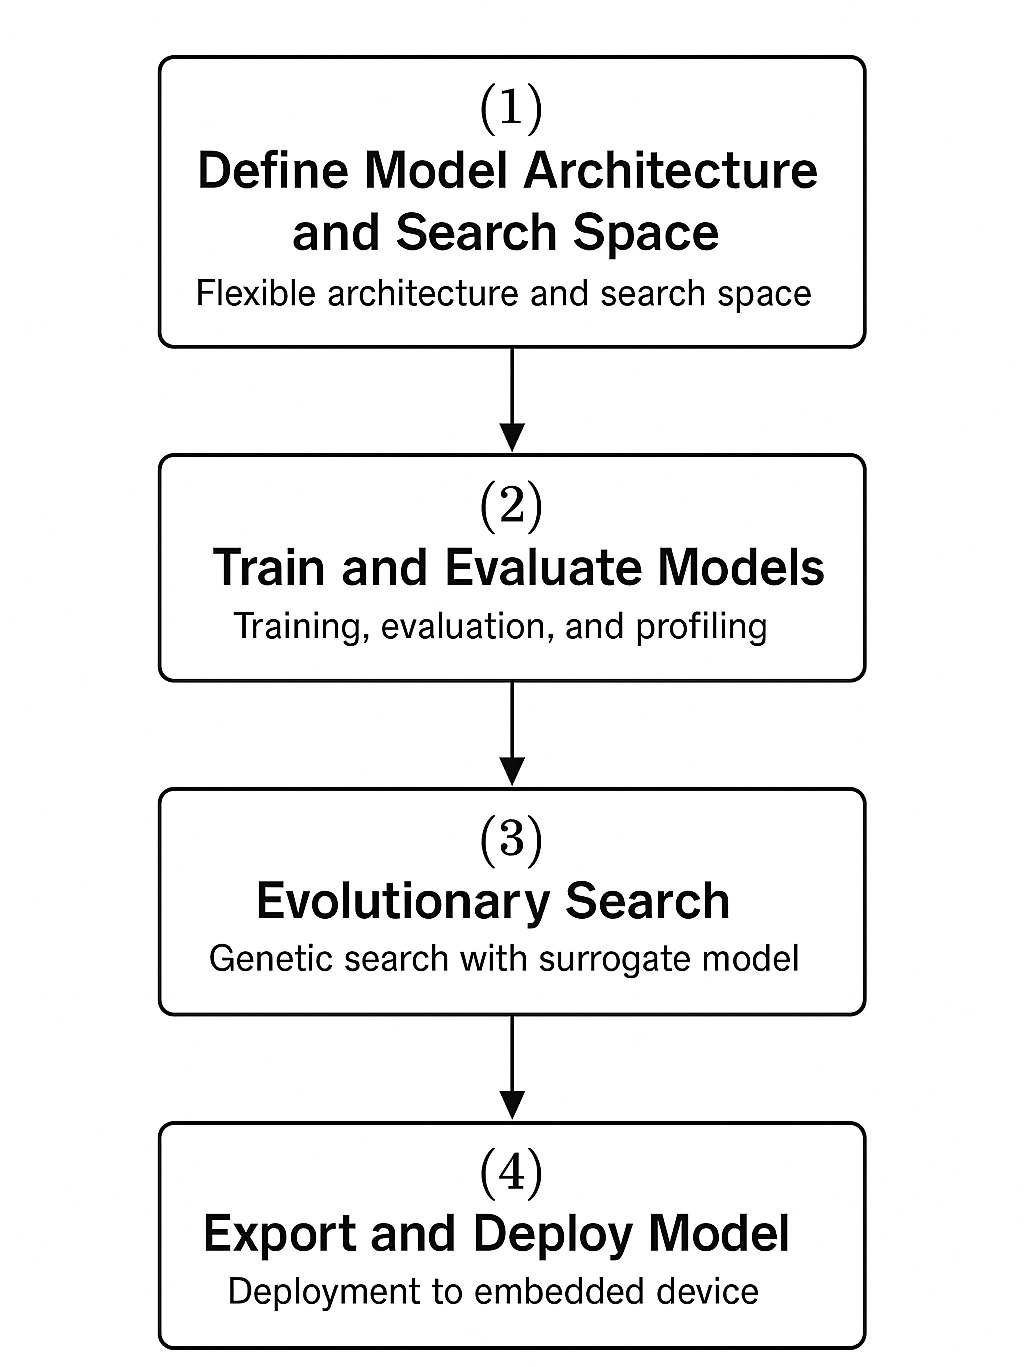
\includegraphics[width=0.6\linewidth]{Pictures/Architegture.png}
    \caption{Architectural pipeline}
    \label{fig:architectural_pipeline}
\end{figure}

\subsection*{Model Creation}

We developed a custom model class \texttt{TakuNetModel} that can construct CNNs from a set of architecture parameters. These parameters (drawn from a predefined search space) define the network’s configuration (e.g., number of layers, kernel sizes etc.). The model is assembled modularly: an initial stem block processes the input, followed by a sequence of repeated stage blocks, and ending with a refiner block that produces the final classification output.

This design allows different architectures to be instantiated by simply varying a configuration dictionary. More about this architecture and the reason it is selected will be explained later.
\TODO{Add Hyperlink to the other Chapter}

\subsection*{Training and Evaluation}

Each trainable model is trained on the CIFAR-100 dataset using TensorFlow 2.x, leveraging GPU acceleration when available.

During training, we record training and validation accuracy. Post-training, the model is evaluated on the test set to compute test accuracy, precision, recall, and F1-score—particularly important for the imbalanced CIFAR-100 dataset. We also profile the model's RAM and flash usage (see Section 3.5) and measure the wall-clock training time for reference.

\subsection*{NAS Evolutionary Loop}

To automate model discovery, we implemented a genetic algorithm. The NAS process maintains a population of candidate models and iteratively evolves them to optimize a multi-objective fitness function (accuracy vs. resource usage).

We begin by sampling an initial population of random architectures from the search space.

Each generation of the evolutionary loop includes:
\begin{enumerate}
    \item \textbf{Parent selection}: Select promising models via tournament selection.
    \item \textbf{Crossover}: Recombine parent architectures to produce offspring.
    \item \textbf{Mutation}: Randomly alter architecture parameters to introduce variation.
\end{enumerate}

This loop runs for a fixed time budget (e.g., 2 hours) or until convergence. After each generation, the best model is recorded. 
At the end of the search, Pareto front analysis is performed to identify architectures that optimally balance accuracy and resource usage. These Pareto-optimal models are saved for reference. 


























\section{Hardware and Software Tools}

Our methodology relies on a combination of software frameworks for machine learning and a target embedded hardware platform. We describe the tools and platforms used below.

\subsection*{TensorFlow and Keras}

We built and trained all neural networks using TensorFlow (version 2.x) with the Keras API. The \texttt{TakuNetModel} class is a Keras \texttt{Model} under the hood, composed of standard Keras layers such as \texttt{Conv2D}, \texttt{DepthwiseConv2D}, and \texttt{Dense}. This choice provided high-level flexibility in defining arbitrary model architectures.

Training was performed on a workstation with GPU support, The GPU used in our experiments was XXXXX.
In addition, we used auxiliary Python libraries: \texttt{scikit-learn} for computing evaluation metrics (precision, recall, F1-score), and \texttt{pandas} for logging results. The genetic algorithm are also implemented in Python using \texttt{NumPy} and \texttt{TensorFlow}. This entire experimentation framework runs offline on a PC.

\subsection*{TensorFlow Lite for Microcontrollers}

To bridge the gap between PC-trained models and deployment on a microcontroller, we used TensorFlow Lite. Specifically, trained models were converted to the TensorFlow Lite FlatBuffer format, and then deployed using TensorFlow Lite for Microcontrollers (TFLite Micro).

TFLite Micro is a lightweight inference engine designed for memory-limited devices. It supports a subset of TensorFlow operators, which influenced our model design to use only supported ops. After training a model in Keras, we used the TFLite converter to produce a quantized \texttt{.tflite} model.

We then developed a utility to convert this binary model into a C array stored in a \texttt{.h} header file. The following Python code illustrates this process:

\begin{lstlisting}[language=Python, caption={Convert a TFLite model to a C header array for Arduino deployment}, label=lst:tflite_to_c_array]
# Convert tflite model to C array for Arduino
with open(f"{self.model_name}.tflite", "rb") as f:
    tflite_bytes = f.read()
c_array = ", ".join(f"0x{b:02x}" for b in tflite_bytes)
model_length = len(tflite_bytes)
header_content = (
    f"#ifndef {self.model_name.upper()}_H\n#define {self.model_name.upper()}_H\n\n"
    f"const unsigned char {self.model_name}_data[{model_length}] = {\n    {c_array}\n}};\n"
    f"const unsigned int {self.model_name}_length = {model_length};\n\n#endif"
)
with open(f"{self.model_name}.h", "w") as header_file:
    header_file.write(header_content)
\end{lstlisting}

This header defines two symbols: an array of bytes with the model data, and a variable with its length. This header is then included in the Arduino project.

On the Arduino side, we use the official TensorFlow Lite Micro library (available through the Arduino Library Manager). The process involves:

\begin{itemize}
    \item Allocating a memory arena (an array of bytes) for use by the TFLite Micro runtime.
    \item Initializing the model interpreter with the model data and memory arena.
    \item Invoking inference on new input data using the interpreter.
\end{itemize}


As a targeted Hardware environment we choose \textbf{Arduino Nano 33 BLE Sense}. More on about the procedure of the deployment will be explain in the relevant chapter.

\TODO{Add Hyperlink to the Deployment Chapter}
